\hypertarget{decomposition-and-mapping-techniques}{%
\section{Decomposition and Mapping
Techniques}\label{decomposition-and-mapping-techniques}}

\begin{itemize}
\tightlist
\item
  identifying portions of the work that can be performed concurrently
  (decomposition)
\item
  mapping the concurrent pieces of work onto multiple processes running
  in parallel
\item
  distributing the input, output, and intermediate data associated with
  the program
\item
  managing accesses to data shared by multiple processors
\item
  synchronizing the processors at various stages of the parallel program
  execution
\end{itemize}

\begin{figure}[H]
\centering
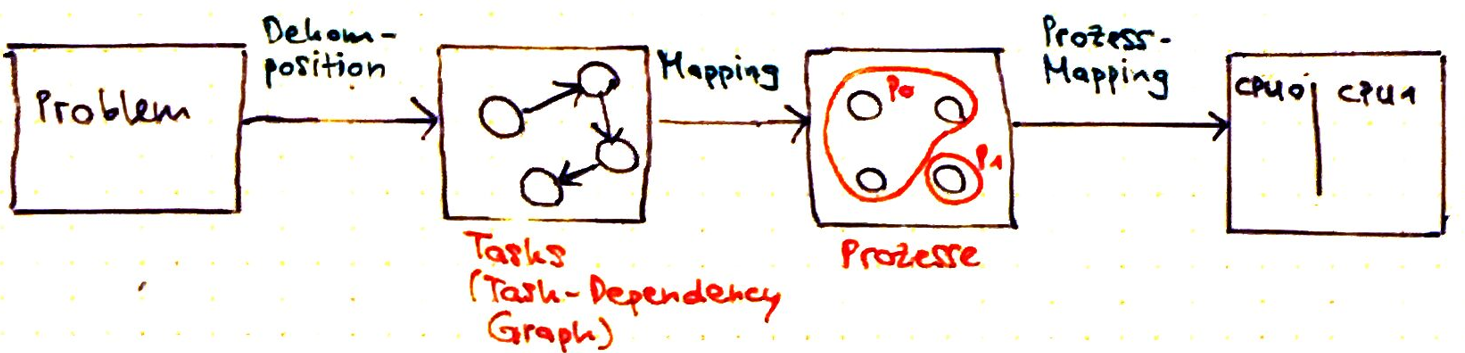
\includegraphics[width=0.7\textwidth]{figures/decomposition.png}
\caption{Decomposition}
\end{figure}

\hypertarget{introduction-to-parallel-algorithms}{%
\subsection{Introduction to Parallel
Algorithms}\label{introduction-to-parallel-algorithms}}

\hypertarget{example-for-a-decomposition}{%
\subsubsection{Example for a
decomposition}\label{example-for-a-decomposition}}

\begin{figure}[H]
\centering
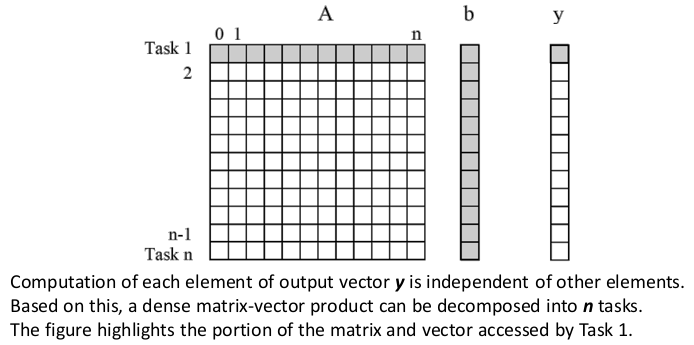
\includegraphics[width=0.7\textwidth]{figures/ExampleVectorMultiplication.png}
\caption{Multiplying Vector Example for decomposition}
\end{figure}

\begin{itemize}
\tightlist
\item
  Every process needs to know b
\item
  Every process gets one row of the matrix
\item
  Every process calucates the scalar of b x and it's row
\end{itemize}

\textit{While tasks share data (namely, the vector b), they do not have
any control dependencies - i.e., no task needs to wait for the (partial)
completion of any other. All tasks are of the same size in terms of
number of operations.}

\hypertarget{degree-of-concurrency}{%
\subsubsection{Degree of Concurrency}\label{degree-of-concurrency}}

\begin{itemize}
\tightlist
\item
  the maximum degree of concurrency is the maximum number of tasks at
  any point during execution
\item
  the average degree of concurrency is the average number of tasks that
  can be processed in parallel over the execution of the program
\item
  the degree of concurrency increases as the decomposition becomes finer
  in granularity and vice versa
\end{itemize}

\begin{tcolorbox}[colback=red!5!white,colframe=red!75!black]
Average degree of concurrency = W / criticalpathlength
\end{tcolorbox}

\hypertarget{critical-path-length}{%
\subsubsection{Critical Path Length}\label{critical-path-length}}

Wie viele Arbeitsschritte dauert die parallele Ausführung mindestens?

\begin{itemize}
\tightlist
\item
  a directed path in the task dependency graph represents a sequence of
  tasks that must be processed one after the other
\item
  the length of the longest path in a task dependency graph is called
  the critical path length (= path with maximum amount of work)
\end{itemize}

\begin{figure}[H]
\centering
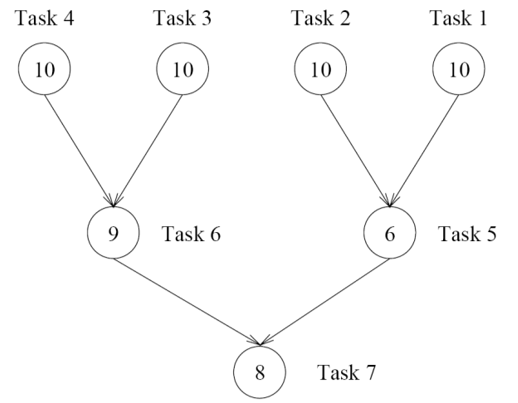
\includegraphics[width=0.35\textwidth]{figures/criticalPathExample.png}
\caption{Critical Path Example}
\end{figure}

In this example, the critical path would be 27. The average degree of
concurrency is 63/27 = 2 1/3.

\clearpage
\hypertarget{task-interaction-graphs}{%
\subsubsection{Task Interaction Graphs}\label{task-interaction-graphs}}

The task interaction graphs represent data dependencies. The task
dependency graphs represent control dependencies.

\begin{itemize}
\tightlist
\item
  For the following example it doesn't make sense to compute the scalar
  for each row, since there are a lot of cells which are 0.
\item
  Each task gets the full row (including b)
\item
  If task 0 wants to compute the scalar, he need to communicate with 1,4
  and 8 (since he need the value of b from them)
\item
  The depencendy graph shows the dependency of each task
\end{itemize}

\begin{figure}[H]
\centering
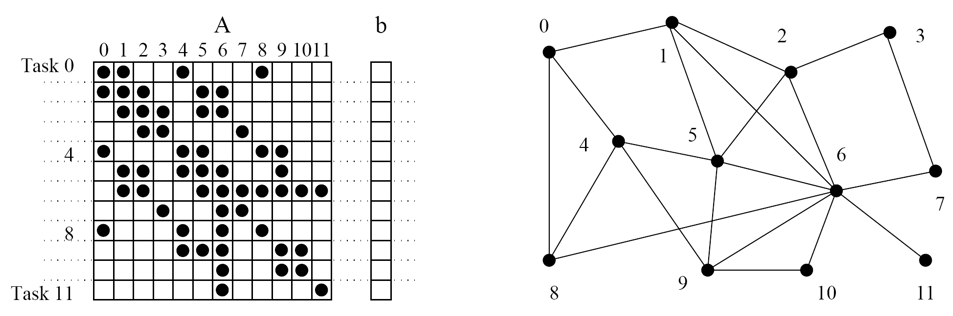
\includegraphics[width=0.7\textwidth]{figures/taskInteractionGraph.png}
\caption{Task Interaction Graph Example}
\end{figure}

\hypertarget{processes-and-mapping}{%
\subsubsection{Processes and Mapping}\label{processes-and-mapping}}

\begin{itemize}
\tightlist
\item
  in general, the number of tasks in a decomposition exceeds the number
  of processing elements available
\item
  for this reason, a parallel algorithm must also provide a mapping of
  tasks to processes
\item
  mappings are determined by both the task dependency and task
  interaction graphs
\end{itemize}

Goals are:

\begin{itemize}
\tightlist
\item
  mapping independent tasks to different processes
\item
  assigning tasks on critical path to processes as soon as they become
  available
\item
  minimizing interaction between processes by mapping tasks with dense
  interactions to the same process
\end{itemize}

\hypertarget{decomposition-techniques}{%
\subsection{Decomposition Techniques}\label{decomposition-techniques}}

How does one decompose a task into various subtasks?

\hypertarget{recursive-decomposition}{%
\subsubsection{Recursive Decomposition}\label{recursive-decomposition}}

\begin{itemize}
\tightlist
\item
  a given problem is first decomposed into a set of sub-problems
\item
  these sub-problems are recursively decomposed further until a desired
  granularity is reached
\end{itemize}

\begin{figure}[H]
\centering
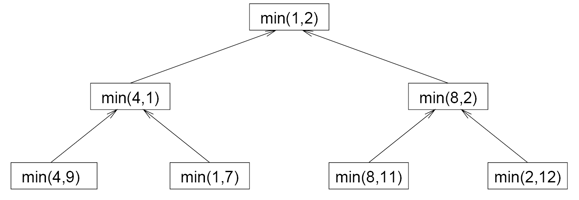
\includegraphics[width=0.5\textwidth]{figures/recursiveExample.png}
\caption{Recursive Example}
\end{figure}

\hypertarget{data-decomposition}{%
\subsubsection{Data Decomposition}\label{data-decomposition}}

\begin{itemize}
\tightlist
\item
  partitions data (input, output, intermediate) used in computations
  across various tasks
\item
  this partitioning induces a decomposition of the problem
\end{itemize}

\hypertarget{input-data-partitioning}{%
\paragraph{Input Data Partitioning}\label{input-data-partitioning}}

\begin{itemize}
\tightlist
\item
  a task is associated with each input data partition
\item
  the task performs as much of the computation with its part of the data
\item
  subsequent processing combines these partial results
\item
  Wird typischerweise verwendet, wenn ein einzelner Output direkt von
  einem einzelnen Input abhängig ist.
\end{itemize}

\hypertarget{output-data-partitioning}{%
\paragraph{Output Data Partitioning}\label{output-data-partitioning}}

\begin{itemize}
\tightlist
\item
  The output elements can be partitioned into different tasks
\item
  e.g.~the computation of the scalar with the example above. Each scalar
  result can be assigned to a different task.
\end{itemize}

\hypertarget{intermediate-data-partitioning}{%
\paragraph{Intermediate Data
Partitioning}\label{intermediate-data-partitioning}}

\begin{itemize}
\tightlist
\item
  computation can often be viewed as a sequence of transformation from
  the input to the output data
\item
  in these cases, it is often beneficial to use one of the intermediate
  stages as a basis for decomposition
\end{itemize}

\hypertarget{exploratory-decomposition}{%
\subsubsection{Exploratory
Decomposition}\label{exploratory-decomposition}}

\begin{itemize}
\tightlist
\item
  the decomposition of the problem goes hand-in-hand with its execution
\item
  these problems typically involve the exploration (search) of a state
  space of solutions
\item
  Often used with graphs or if you know the number of tasks just by
  runtime
\end{itemize}

\hypertarget{mapping-techniques-for-load-balancing}{%
\subsection{Mapping Techniques for Load
Balancing}\label{mapping-techniques-for-load-balancing}}

\begin{itemize}
\tightlist
\item
  Das Mapping sollte gleichzeitig dafür sorgen, dass wir ein gutes
  Load-Balancing haben und darauf achten, dass einzelne Prozesse in
  einem Warte-Zustand sind.
\item
  Mit dem Mapping versuchen wir zu erreichen, dass wir kosten-optimal
  sind.
\end{itemize}

\hypertarget{static-mapping}{%
\subsubsection{Static Mapping}\label{static-mapping}}

\begin{itemize}
\tightlist
\item
  tasks are mapped to processes a-priori
\item
  we must have a good estimate of the size of each task
\item
  finding an optimum might be NP complete
\end{itemize}

\hypertarget{dynamic-mapping-dynamic-load-balancing}{%
\subsubsection{Dynamic Mapping (Dynamic Load
Balancing)}\label{dynamic-mapping-dynamic-load-balancing}}

\begin{itemize}
\tightlist
\item
  tasks are mapped to processes at runtime
\item
  static mapping is not possible, because the tasks are generated at
  runtime or their sizes are unknown
\end{itemize}

\hypertarget{mapping-schemes}{%
\subsubsection{Mapping Schemes}\label{mapping-schemes}}

\begin{itemize}
\tightlist
\item
  Schemes for Static Mapping

  \begin{itemize}
  \tightlist
  \item
    mappings based on data partitioning
  \item
    mappings based on task graph partitioning
  \item
    hybrid mappings
  \end{itemize}
\item
  Schemes for Dynamic Mapping

  \begin{itemize}
  \tightlist
  \item
    centralized

    \begin{itemize}
    \tightlist
    \item
      managed by a master
    \item
      slaves that run out of work request the master for more work
    \end{itemize}
  \item
    distributed

    \begin{itemize}
    \tightlist
    \item
      each process can send or receive work from other processes
    \item
      eliminates the bottleneck of centralized schemes, but has also
      some hazards
    \end{itemize}
  \end{itemize}
\end{itemize}

\clearpage
\hypertarget{block-array-distribution-schemes}{%
\paragraph{Block Array Distribution
Schemes}\label{block-array-distribution-schemes}}

\begin{itemize}
\tightlist
\item
  The following shows the advantage of a block array distribution scheme
  when multiplying two matrices
\item
  the choice of precise decomposition (1-D or 2-D) is determined by the
  associated communication overhead
\item
  with the chosen blocks, not all processors need to know the whole B
\end{itemize}

\begin{figure}[H]
\centering
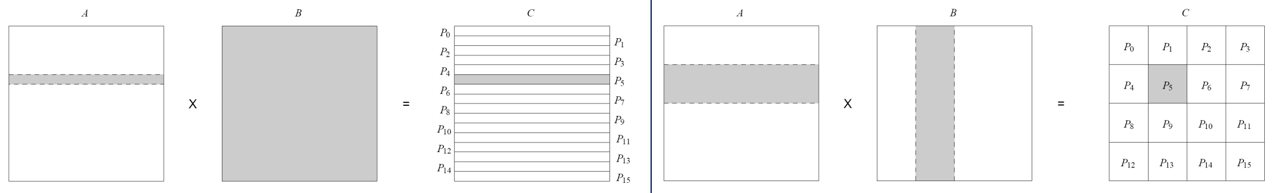
\includegraphics[width=1\textwidth]{figures/blockdistributionscheme.png}
\caption{Block Array Distribution Scheme Example}
\end{figure}

\hypertarget{block-cyclic-distributions}{%
\paragraph{(Block) Cyclic
Distributions}\label{block-cyclic-distributions}}

\begin{itemize}
\tightlist
\item
  variation of the block distribution scheme that can be used to
  alleviate the load-imbalance and idling problems
\item
  blocks are assigned to processes in a round-robin manner so that each
  process gets several non-adjacent blocks
\end{itemize}

\hypertarget{solving-a-system-of-linear-equations}{%
\subsubsection{Solving a System of Linear
Equations}\label{solving-a-system-of-linear-equations}}

\begin{itemize}
\tightlist
\item
  We are searching for an algorithm which solves the system of linear
  equation Ax = b

  \begin{itemize}
  \tightlist
  \item
    We know A and b
  \item
    We search for x
  \end{itemize}
\item
  This can be done with the Gaussian Elimination Algorithm (LU
  decomposition)
\end{itemize}

\begin{figure}[H]
\centering
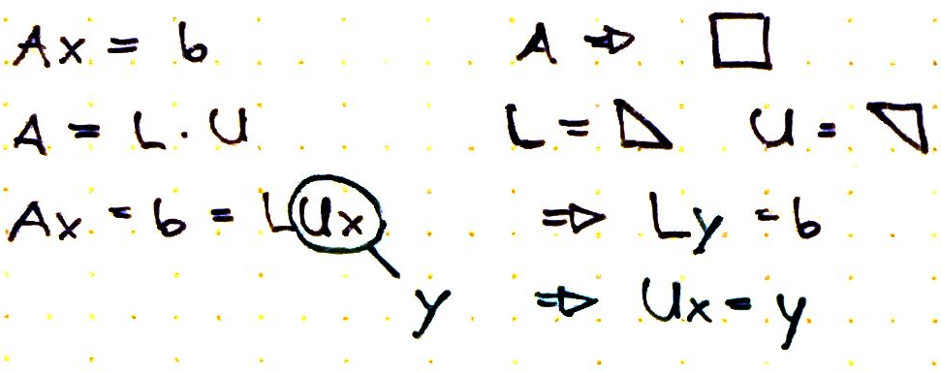
\includegraphics[width=0.7\textwidth]{figures/linearEquations.png}
\caption{Solving System of linear equations}
\end{figure}

\begin{figure}[H]
\centering
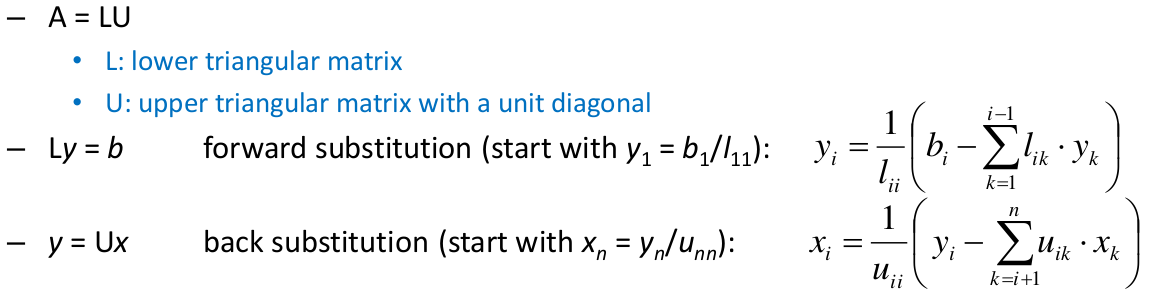
\includegraphics[width=0.8\textwidth]{figures/LU1.png}
\caption{LU approach}
\end{figure}

\begin{figure}[H]
\centering
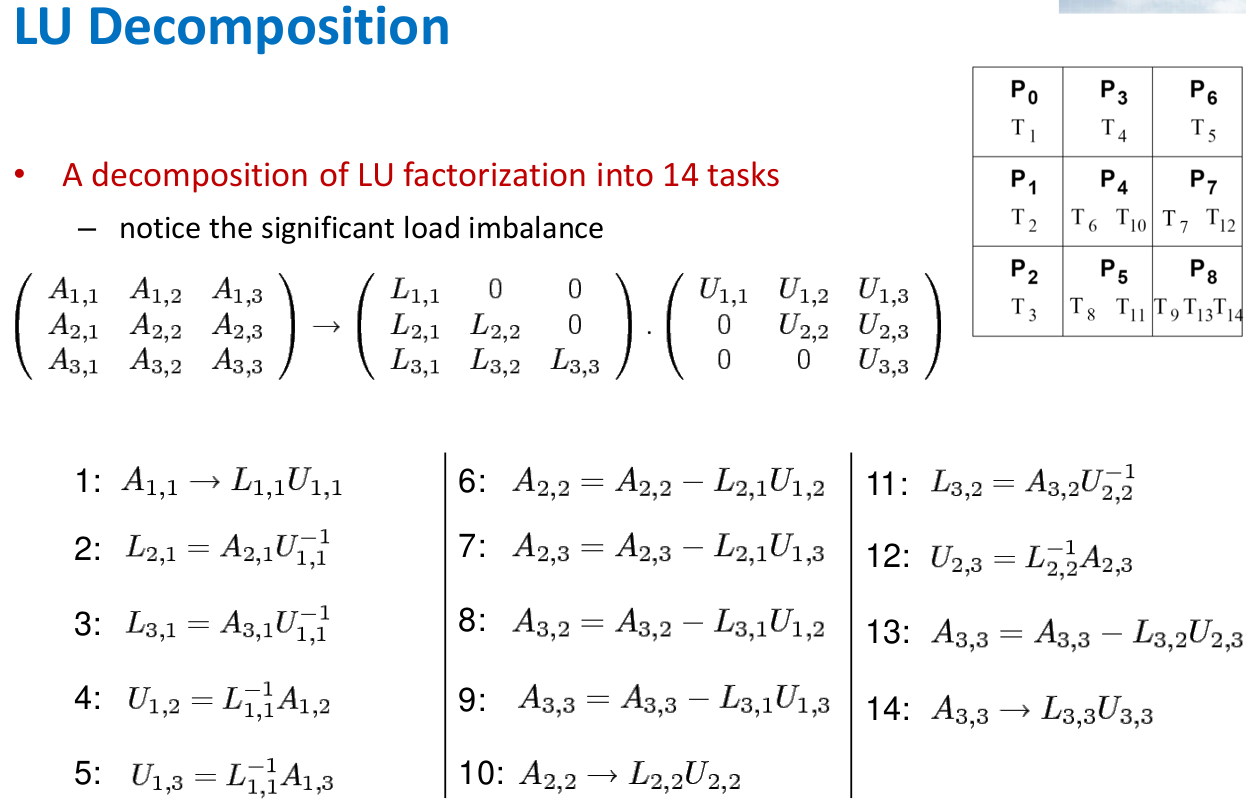
\includegraphics[width=0.8\textwidth]{figures/LU2.png}
\caption{LU Decomposition}
\end{figure}

\begin{figure}[H]
\centering
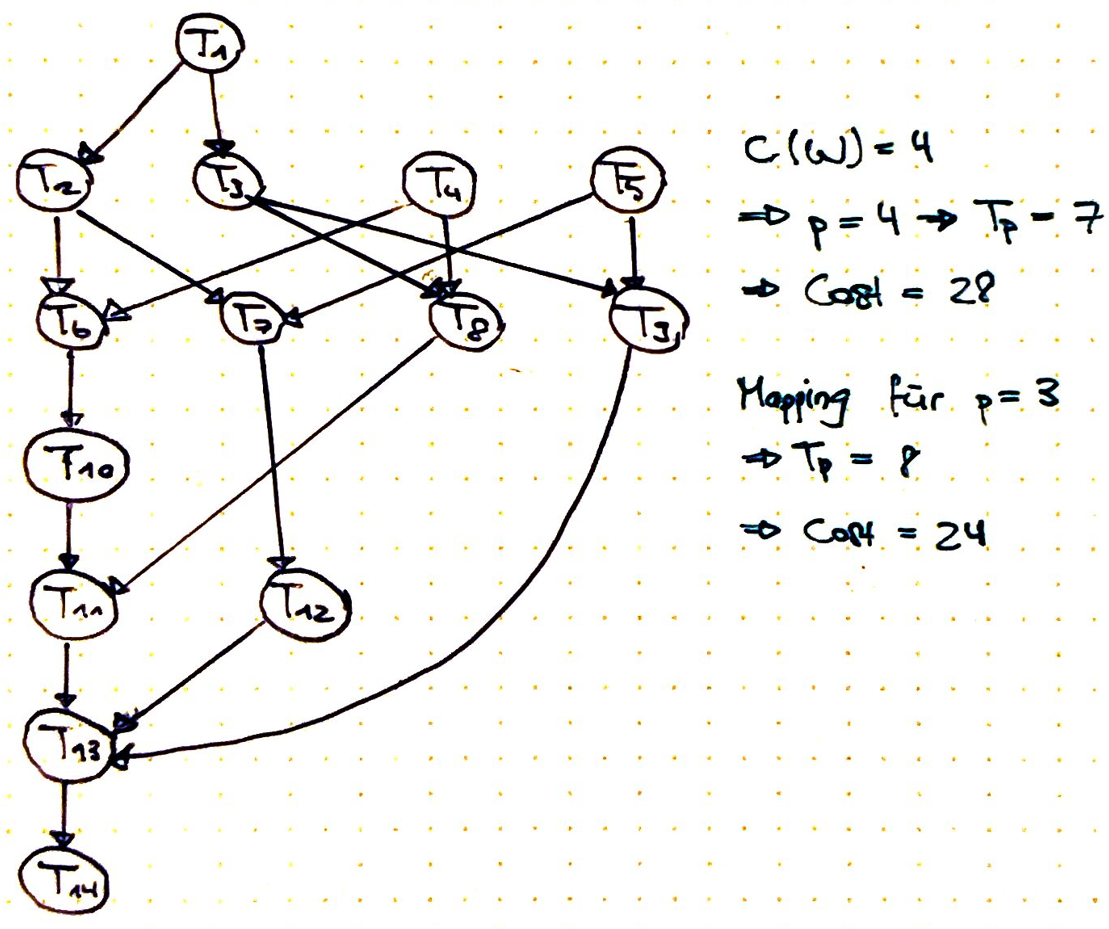
\includegraphics[width=0.5\textwidth]{figures/dependencyGraph.png}
\caption{Dependency Graph}
\end{figure}

\clearpage